\documentclass[letterpaper, 10pt, twoside]{article}
\usepackage[english]{babel} % English language/hyphenation
\usepackage[utf8]{inputenc} % Use all the utf8 characters

\usepackage{amsmath} % Math packages
\usepackage{amsfonts} % Math packages
\usepackage{amsthm} % Math packages
\usepackage{physics} % Physics packages
\usepackage{graphicx} 

\usepackage[hmarginratio=1:1,top=32mm,columnsep=20pt,right=1in,left=1in]{geometry} % Document margins

\usepackage{titlesec} % Allows customization of titles

\usepackage{hyperref} % For hyperlinks in the PDF

\titleformat{\section}[block]{\large\scshape\centering}{\thesection.}{1em}{} % Change the look of the section titles
\titleformat{\subsection}[block]{\large}{\thesubsection.}{1em}{} % Change the look of the section titles
\newcommand{\horrule}[1]{\rule{\linewidth}{#1}} % Create horizontal rule command with 1 argument of height
\usepackage{fancyhdr} % Headers and footers
\pagestyle{fancy} % All pages have headers and footers
\fancyhead{} % Blank out the default header
\fancyfoot{} % Blank out the default footer

\fancyhead[C]{UC Berkeley $\bullet$ title $\bullet$ Author} % Custom header text

\fancyfoot[C]{\thepage} % Custom footer text


\usepackage[caption=false]{subfig}


\title{\vspace{-19mm}Pending title}
\author{Leonard Harkins}
\date{\today}

\begin{document}

\maketitle
\thispagestyle{fancy}

\section{Task 1}

In this first task you will be looking at the value of the integral
\input{task1_equations}

\begin{figure}[htbp!]
\hfil
\subfloat[\label{fig:2.1}Caption2.1.]{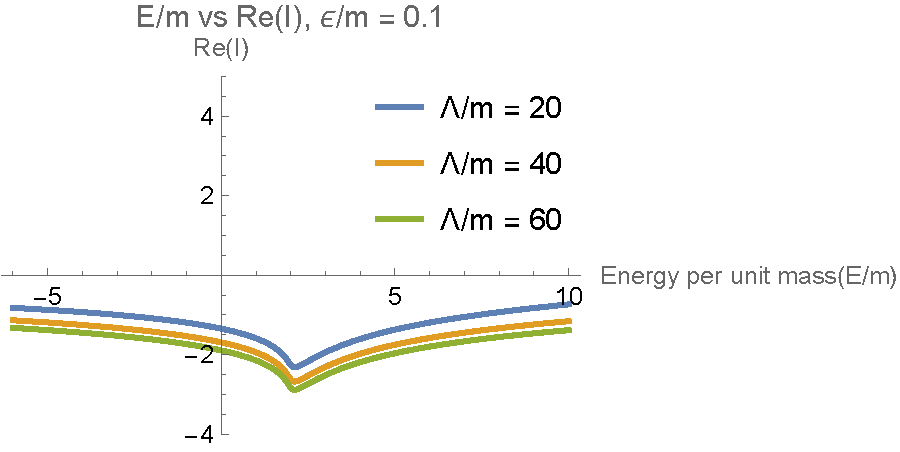
\includegraphics[width=0.5\linewidth]{task1_plots/E_vs_Re_I_epsilon_01.pdf}}
\hfil
\subfloat[\label{fig:2.2}Caption2.2.]{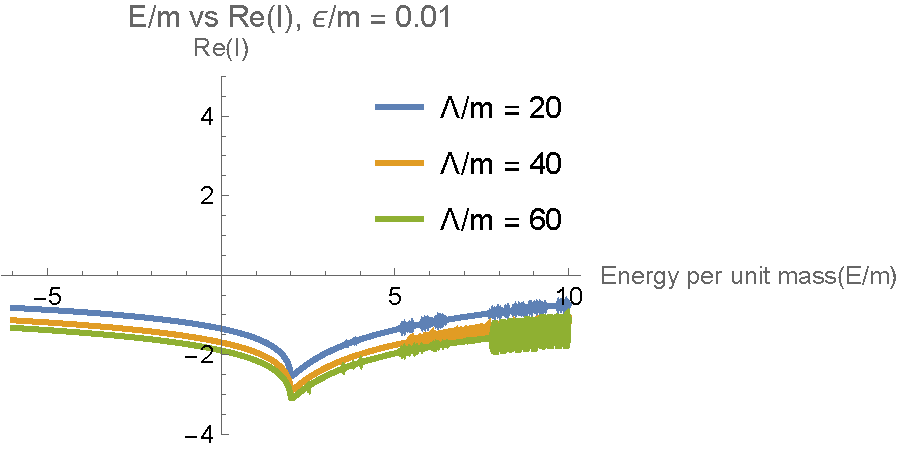
\includegraphics[width=0.5\linewidth]{task1_plots/E_vs_Re_I_epsilon_001.pdf}}
\hfil
\subfloat[\label{fig:2.2}Caption2.3.]{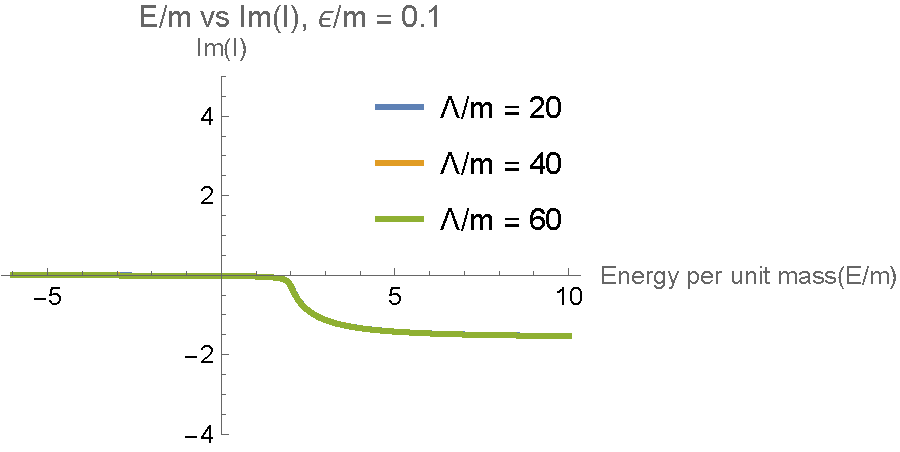
\includegraphics[width=0.5\linewidth]{task1_plots/E_vs_Im_I_epsilon_01.pdf}}
\hfil
\subfloat[\label{fig:2.2}Caption2.4.]{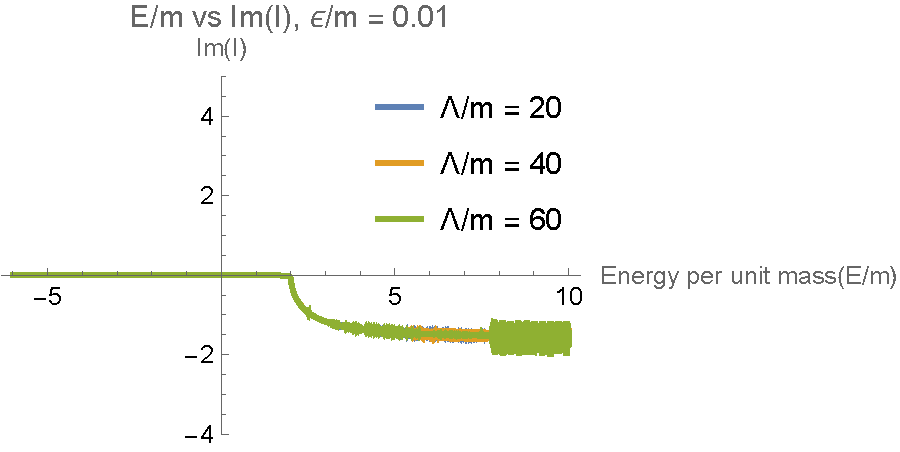
\includegraphics[width=0.5\linewidth]{task1_plots/E_vs_Im_I_epsilon_001.pdf}}
\hfil
%Don't leave a line between subfloats if they should appear on the same line.
\caption{\label{fig:2}Caption2.}
\end{figure}

Integral simplification:
\begin{align}
    I(E,m,\epsilon) = \int^\Lambda_0 \frac{d^3\vec{k}}{(2\pi)^3} \frac{1}{(2\omega_k)^2(E-2\omega_k+i\epsilon)}\\
    I(E,m,\epsilon) = \int^\Lambda_0 \frac{4 \pi k^2 dk}{(2\pi)^3} \frac{1}{4(k^2+m^2)^2(E-2\sqrt{k^2+m^2}+i\epsilon)}\\
    I(E,m,\epsilon) = \int^{\Lambda/m}_0 \frac{\pi x^2 dx}{(2\pi)^3(x^2+1)^2(E/m-2\sqrt{x^2+1}+i\epsilon/m)}\\
\end{align}


Analytically taking the limit as $\epsilon \to 0$:
\begin{equation}
    \lim_{\epsilon \to 0} \int^{\Lambda/m}_0 \frac{\pi x^2 dx}{(2\pi)^3(x^2+1)^2}\frac{1}{(E/m-2\sqrt{x^2+1}+i\epsilon/m)}\,,
\end{equation}
using the identity:
\begin{align}    
\lim_{\epsilon \to 0^+} \frac{1}{x+i\epsilon} &= P(\frac{1}{x}) - i\pi\delta(x)\\
     &\int^{\Lambda/m}_0 (\frac{\pi x^2 dx}{(2\pi)^3(x^2+1)^2})
     \left(P\frac{1}{E/m-2\sqrt{x^2+1}} - i\pi\delta(E/m-2\sqrt{x^2+1})\right)\,,
\end{align}
using the identity:
\begin{equation}
\delta(g(x)) = \sum_{i} \frac{\delta(x-x_i)}{|g'(x_i)|}
\end{equation}
where $x_i$ are the roots of $g(x)$. The roots are found as follows, keeping in mind that $x_i$ must be real as we are integrating only over real values of x: 
\begin{align}
g(x) = E/m-2\sqrt{x^2+1}\\
E/m-2\sqrt{x_i^2+1} = 0, E/m \ge 2\\
x_i = \pm\frac{1}{2}\sqrt{\left(\frac{E}{m}\right)^2-4}, E/m \ge 2\\
|g'(x)| = \frac{2x}{\sqrt{x^2+1}}\\
|g'(x_i)| = \frac{2m\sqrt{\left(\frac{E}{m}\right)^2-4}}{E}, E/m \ge 2\\
\delta(E/m - 2\sqrt{x^2+1}) = \frac{E}{2m\sqrt{\left(\frac{E}{m}\right)^2-4}}(\delta(x-\frac{1}{2}\sqrt{(E/m)^2 - 4}) + \delta(x+\frac{1}{2}\sqrt{(E/m)^2 - 4}))\Theta(E/m-2)
\end{align}
We keep only the first delta function which has a nonzero integral over $[0,\Lambda/m]$ and multiply by the Heaviside step function to enforce $E/m \ge 2$ which results from x being real. Plugging back into the integral we arrive at an analytic solution to the imaginary component.
\begin{align}
     \int^{\Lambda/m}_0 P(\frac{\pi x^2 dx}{(2\pi)^3(x^2+1)^2}\frac{1}{E/m-2\sqrt{x^2+1}}) -  \int^{\Lambda/m}_0 \frac{\pi x^2 dx}{(2\pi)^3(x^2+1)^2}\frac{i\pi E\delta(x-\frac{1}{2}\sqrt{(E/m)^2 - 4})}{2m\sqrt{(E/m)^2 - 4}})\Theta(E/m-2)
\end{align}
\begin{align}
     \int^{\Lambda/m}_0 P(\frac{\pi x^2 dx}{(2\pi)^3(x^2+1)^2}\frac{1}{E/m-2\sqrt{x^2+1}}) - \frac{i\pi^2}{(2\pi)^3}\frac{\sqrt{(E/m)^2-4}}{2(E/m)^2}\Theta(E/m-2)
\end{align}

\begin{figure}[htbp!]
\hfil
\subfloat[\label{fig:2.1}Caption2.1.]{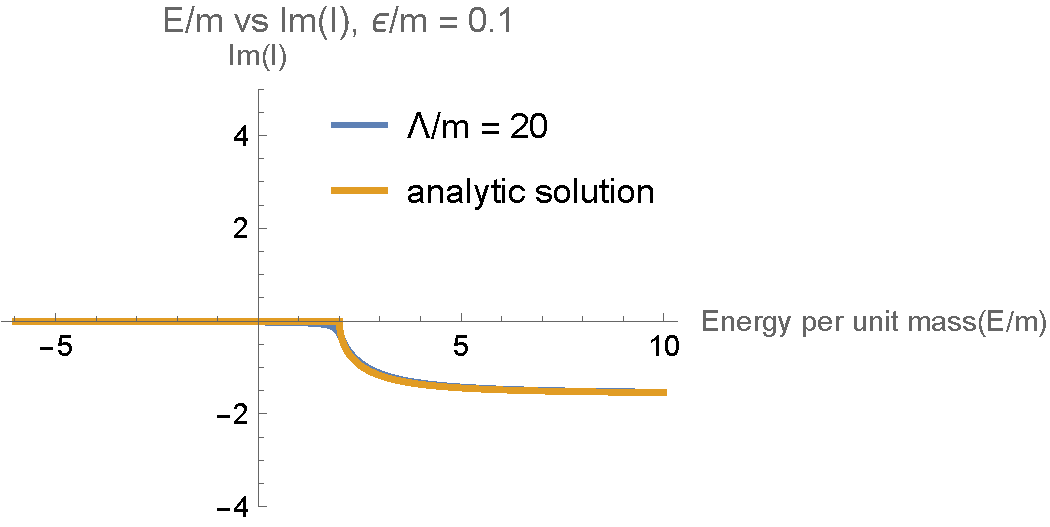
\includegraphics[width=0.5\linewidth]{task1_plots/E_vs_Im_I_epsilon_01_analytic_solution.pdf}}
\hfil
\subfloat[\label{fig:2.2}Caption2.2.]{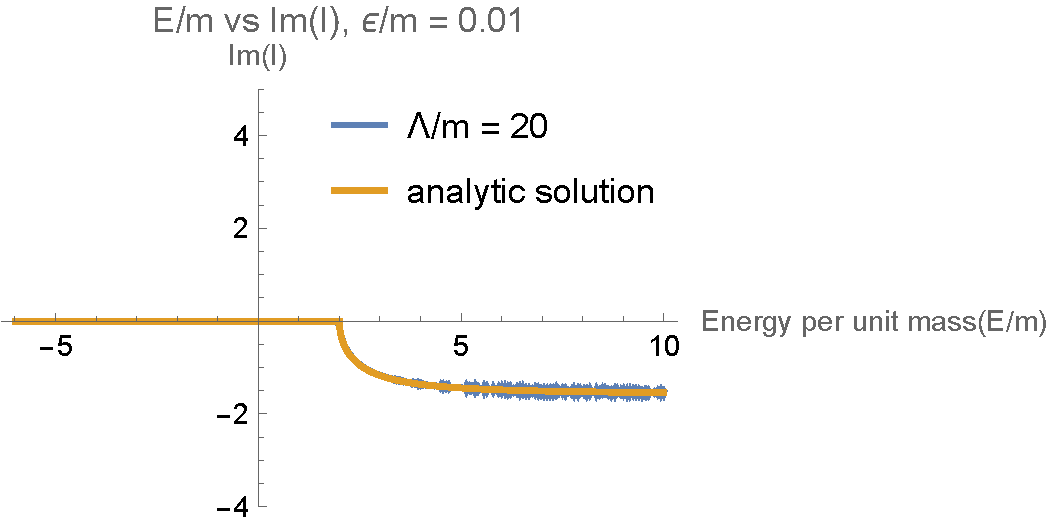
\includegraphics[width=0.5\linewidth]{task1_plots/E_vs_Im_I_epsilon_001_analytic_solution.pdf}}
\hfil
\subfloat[\label{fig:2.2}Caption2.3.]{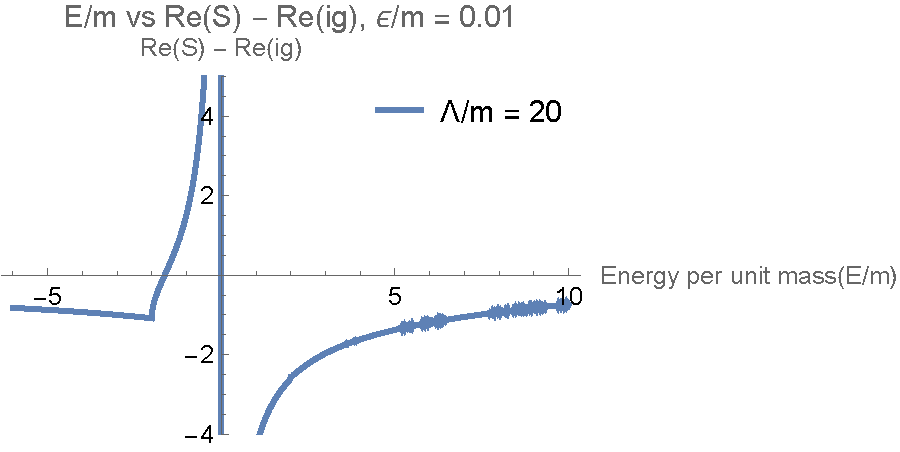
\includegraphics[width=0.5\linewidth]{task1_plots/E_vs_Re_I_minus_Re_ig_epsilon_001.pdf}}
\hfil
%Don't leave a line between subfloats if they should appear on the same line.
\caption{\label{fig:2}Caption2.}
\end{figure}

\section{Task 2}

In this second task you will be looking at the value of the integral
\begin{align}
I(E_f, E_i, q_0, m) = \int \frac{d k_0 \, d^3 \vec{k}}{(2\pi)^4}
\frac{1}{
\left[(E_f - k_0)^2 - \omega_k^2 + i\epsilon\right]
\left[(q_0 + E_f - k_0)^2 - \omega_k^2 + i\epsilon\right]
\left[(E_i - k_0)^2 - \omega_k^2 + i\epsilon\right]
\left[(k_0)^2 - \omega_k^2 + i\epsilon\right]
}\,,
\end{align}
\begin{align}
\omega_k &= \sqrt{|\vec{k}|^2+m^2}
\end{align}

Integral simplification: 
to evaluate the contour integral over $k_0$ with the residue theorem, we need all the poles enclosed in the contour. $\int d k_0 = 2 \pi i \sum (\text{residues})$
\begin{align}
(E_f - k_0)^2 - \omega_k^2 + i\epsilon = 0\\
\text{poles 1 and 2: } k_0 = E_f \pm (\omega_k -i \epsilon)\\
(q_0 + E_f - k_0)^2 - \omega_k^2 + i\epsilon = 0\\
\text{poles 3 and 4: } k_0 = q_0 E_f \pm (\omega_k -i \epsilon)\\
(E_i - k_0)^2 - \omega_k^2 + i\epsilon = 0\\
\text{poles 5 and 6: } k_0 = E_i \pm (\omega_k -i \epsilon)\\
(k_0)^2 - \omega_k^2 + i\epsilon = 0\\
\text{poles 7 and 8: }k_0 =\pm (\omega_k -i \epsilon)
\end{align}
We only keep the poles with $-i \epsilon$ for the residues: $Res(f, c) = \lim_{x\to c} (x-c) f$, where c is a pole.
\begin{align*}
&I(E_f, E_i, q_0, m) = \\
&\left[
\lim_{k_0 \to E_f + \omega_k - i \epsilon} (k_0 - E_f - \omega_k + i \epsilon)
+ \lim_{k_0 \to q_0 + E_f + \omega_k - i \epsilon} (k_0 - q_0 - E_f - \omega_k + i \epsilon) \right. \\
&\quad + \lim_{k_0 \to E_i + \omega_k - i \epsilon} (k_0 - E_i - \omega_k + i \epsilon)
+ \left. \lim_{k_0 \to \omega_k - i \epsilon} (k_0 - \omega_k + i \epsilon) \right] \\
&\quad \times \int \frac{d^3 \vec{k}}{(2\pi)^4}
\frac{1}{
\left[(E_f - k_0)^2 - \omega_k^2 + i\epsilon\right]
\left[(q_0 + E_f - k_0)^2 - \omega_k^2 + i\epsilon\right]
\left[(E_i - k_0)^2 - \omega_k^2 + i\epsilon\right]
\left[k_0^2 - \omega_k^2 + i\epsilon\right]
}\,.
\end{align*}
\begin{align*}
&I(E_f, E_i, q_0, m) = \\
&\int \frac{d^3 \vec{k}}{(2\pi)^4} \times\\
&\bigg(\lim_{k_0 \to E_f + \omega_k - i \epsilon}\quad\frac{(k_0 - E_f - \omega_k + i \epsilon)}{
\left[(E_f - k_0)^2 - \omega_k^2 + i\epsilon\right]
\left[(q_0 + E_f - k_0)^2 - \omega_k^2 + i\epsilon\right]
\left[(E_i - k_0)^2 - \omega_k^2 + i\epsilon\right]
\left[k_0^2 - \omega_k^2 + i\epsilon\right]
} \\
&\quad + \lim_{k_0 \to q_0 + E_f + \omega_k - i \epsilon}\frac{(k_0 - q_0 - E_f - \omega_k + i \epsilon)}{
\left[(E_f - k_0)^2 - \omega_k^2 + i\epsilon\right]
\left[(q_0 + E_f - k_0)^2 - \omega_k^2 + i\epsilon\right]
\left[(E_i - k_0)^2 - \omega_k^2 + i\epsilon\right]
\left[k_0^2 - \omega_k^2 + i\epsilon\right]
} \\
&\quad + \lim_{k_0 \to E_i + \omega_k - i \epsilon}\frac{(k_0 - E_i - \omega_k + i \epsilon)}{
\left[(E_f - k_0)^2 - \omega_k^2 + i\epsilon\right]
\left[(q_0 + E_f - k_0)^2 - \omega_k^2 + i\epsilon\right]
\left[(E_i - k_0)^2 - \omega_k^2 + i\epsilon\right]
\left[k_0^2 - \omega_k^2 + i\epsilon\right]
} \\
&\quad + \lim_{k_0 \to \omega_k - i \epsilon}\frac{(k_0 - \omega_k + i \epsilon)}{
\left[(E_f - k_0)^2 - \omega_k^2 + i\epsilon\right]
\left[(q_0 + E_f - k_0)^2 - \omega_k^2 + i\epsilon\right]
\left[(E_i - k_0)^2 - \omega_k^2 + i\epsilon\right]
\left[k_0^2 - \omega_k^2 + i\epsilon\right]
} \bigg)
\end{align*}
\begin{align*}
&I(E_f, E_i, q_0, m) = \\
&\int \frac{d^3 \vec{k}}{(2\pi)^4} \times\\
&\bigg(\lim_{k_0 \to E_f + \omega_k - i \epsilon}\quad\frac{(k_0 - E_f - \omega_k + i \epsilon)}{
\left[(k_0 -E_f)^2 - (\sqrt{\omega_k^2 - i\epsilon})^2\right] %
\left[(q_0 + E_f - k_0)^2 - \omega_k^2 + i\epsilon\right]
\left[(E_i - k_0)^2 - \omega_k^2 + i\epsilon\right]
\left[k_0^2 - \omega_k^2 + i\epsilon\right]
} \\
&\quad + \lim_{k_0 \to q_0 + E_f + \omega_k - i \epsilon}\frac{(k_0 - q_0 - E_f - \omega_k + i \epsilon)}{
\left[(E_f - k_0)^2 - \omega_k^2 + i\epsilon\right]
\left[(k_0 -q_0 - E_f)^2 - (\sqrt{\omega_k^2 - i\epsilon})^2\right]%
\left[(E_i - k_0)^2 - \omega_k^2 + i\epsilon\right]
\left[k_0^2 - \omega_k^2 + i\epsilon\right]
} \\
&\quad + \lim_{k_0 \to E_i + \omega_k - i \epsilon}\frac{(k_0 - E_i - \omega_k + i \epsilon)}{
\left[(E_f - k_0)^2 - \omega_k^2 + i\epsilon\right]
\left[(q_0 + E_f - k_0)^2 - \omega_k^2 + i\epsilon\right]
\left[(k_0 - E_i)^2 - (\sqrt{\omega_k^2 - i\epsilon})^2\right]%
\left[k_0^2 - \omega_k^2 + i\epsilon\right]
} \\
&\quad + \lim_{k_0 \to \omega_k - i \epsilon}\frac{(k_0 - \omega_k + i \epsilon)}{
\left[(E_f - k_0)^2 - \omega_k^2 + i\epsilon\right]
\left[(q_0 + E_f - k_0)^2 - \omega_k^2 + i\epsilon\right]
\left[(E_i - k_0)^2 - \omega_k^2 + i\epsilon\right]
\left[k_0^2 - (\sqrt{\omega_k^2 - i\epsilon})^2\right]%
} \bigg)
\end{align*}
using the first order Taylor expansion for small $\epsilon$:$\sqrt{\omega_k^2 - i \epsilon} = \omega_k - i \epsilon$
\begin{align*}
&I(E_f, E_i, q_0, m) = \\
&\int \frac{d^3 \vec{k}}{(2\pi)^4} \times\\
&\bigg(\lim_{k_0 \to E_f + \omega_k - i \epsilon}\quad\frac{(k_0 - E_f - \omega_k + i \epsilon)}{
\left[(k_0 -E_f)^2 - (\omega_k - i \epsilon)^2\right] %
\left[(q_0 + E_f - k_0)^2 - \omega_k^2 + i\epsilon\right]
\left[(E_i - k_0)^2 - \omega_k^2 + i\epsilon\right]
\left[k_0^2 - \omega_k^2 + i\epsilon\right]
} \\
&\quad + \lim_{k_0 \to q_0 + E_f + \omega_k - i \epsilon}\frac{(k_0 - q_0 - E_f - \omega_k + i \epsilon)}{
\left[(E_f - k_0)^2 - \omega_k^2 + i\epsilon\right]
\left[(k_0 -q_0 - E_f)^2 - (\omega_k - i \epsilon)^2\right]%
\left[(E_i - k_0)^2 - \omega_k^2 + i\epsilon\right]
\left[k_0^2 - \omega_k^2 + i\epsilon\right]
} \\
&\quad + \lim_{k_0 \to E_i + \omega_k - i \epsilon}\frac{(k_0 - E_i - \omega_k + i \epsilon)}{
\left[(E_f - k_0)^2 - \omega_k^2 + i\epsilon\right]
\left[(q_0 + E_f - k_0)^2 - \omega_k^2 + i\epsilon\right]
\left[(k_0 - E_i)^2 - (\omega_k - i \epsilon)^2\right]%
\left[k_0^2 - \omega_k^2 + i\epsilon\right]
} \\
&\quad + \lim_{k_0 \to \omega_k - i \epsilon}\frac{(k_0 - \omega_k + i \epsilon)}{
\left[(E_f - k_0)^2 - \omega_k^2 + i\epsilon\right]
\left[(q_0 + E_f - k_0)^2 - \omega_k^2 + i\epsilon\right]
\left[(E_i - k_0)^2 - \omega_k^2 + i\epsilon\right]
\left[k_0^2 - (\omega_k - i \epsilon)^2\right]%
} \bigg)
\end{align*}
Using difference of squares (bad alignment - fix later):
\begin{align*}
&I(E_f, E_i, q_0, m) = \\
&\int \frac{d^3 \vec{k}}{(2\pi)^4} \times\\
&\bigg(\lim_{k_0 \to E_f + \omega_k - i \epsilon}\quad\frac{(k_0 - E_f - \omega_k + i \epsilon)}{
\left[k_0 -E_f - \omega_k + i \epsilon\right] %
\left[k_0 -E_f + \omega_k - i \epsilon\right]
\left[(q_0 + E_f - k_0)^2 - \omega_k^2 + i\epsilon\right]
\left[(E_i - k_0)^2 - \omega_k^2 + i\epsilon\right]
\left[k_0^2 - \omega_k^2 + i\epsilon\right]
} \\
&\quad + \lim_{k_0 \to q_0 + E_f + \omega_k - i \epsilon}\frac{(k_0 - q_0 - E_f - \omega_k + i \epsilon)}{
\left[(E_f - k_0)^2 - \omega_k^2 + i\epsilon\right]
\left[k_0 -q_0 - E_f - \omega_k + i \epsilon\right]%
\left[k_0 -q_0 - E_f + \omega_k - i \epsilon\right]%
\left[(E_i - k_0)^2 - \omega_k^2 + i\epsilon\right]
\left[k_0^2 - \omega_k^2 + i\epsilon\right]
} \\
&\quad + \lim_{k_0 \to E_i + \omega_k - i \epsilon}\frac{(k_0 - E_i - \omega_k + i \epsilon)}{
\left[(E_f - k_0)^2 - \omega_k^2 + i\epsilon\right]
\left[(q_0 + E_f - k_0)^2 - \omega_k^2 + i\epsilon\right]
\left[k_0 - E_i - \omega_k + i \epsilon\right]%
\left[k_0 - E_i + \omega_k - i \epsilon\right]%
\left[k_0^2 - \omega_k^2 + i\epsilon\right]
} \\
&\quad + \lim_{k_0 \to \omega_k - i \epsilon}\frac{(k_0 - \omega_k + i \epsilon)}{
\left[(E_f - k_0)^2 - \omega_k^2 + i\epsilon\right]
\left[(q_0 + E_f - k_0)^2 - \omega_k^2 + i\epsilon\right]
\left[(E_i - k_0)^2 - \omega_k^2 + i\epsilon\right]
\left[k_0 - \omega_k + i \epsilon\right]%
\left[k_0 + \omega_k - i \epsilon\right]%
} \bigg)
\end{align*}
And then canceling numerators: 
\begin{align*}
&I(E_f, E_i, q_0, m) = \\
&\int \frac{d^3 \vec{k}}{(2\pi)^4} \times\\
&\bigg(\lim_{k_0 \to E_f + \omega_k - i \epsilon}\quad\frac{1}{
\left[k_0 -E_f + \omega_k - i \epsilon\right]
\left[(q_0 + E_f - k_0)^2 - \omega_k^2 + i\epsilon\right]
\left[(E_i - k_0)^2 - \omega_k^2 + i\epsilon\right]
\left[k_0^2 - \omega_k^2 + i\epsilon\right]
} \\
&\quad + \lim_{k_0 \to q_0 + E_f + \omega_k - i \epsilon}\frac{1}{
\left[(E_f - k_0)^2 - \omega_k^2 + i\epsilon\right]
\left[k_0 -q_0 - E_f + \omega_k - i \epsilon\right]%
\left[(E_i - k_0)^2 - \omega_k^2 + i\epsilon\right]
\left[k_0^2 - \omega_k^2 + i\epsilon\right]
} \\
&\quad + \lim_{k_0 \to E_i + \omega_k - i \epsilon}\frac{1}{
\left[(E_f - k_0)^2 - \omega_k^2 + i\epsilon\right]
\left[(q_0 + E_f - k_0)^2 - \omega_k^2 + i\epsilon\right]
\left[k_0 - E_i + \omega_k - i \epsilon\right]%
\left[k_0^2 - \omega_k^2 + i\epsilon\right]
} \\
&\quad + \lim_{k_0 \to \omega_k - i \epsilon}\frac{1}{
\left[(E_f - k_0)^2 - \omega_k^2 + i\epsilon\right]
\left[(q_0 + E_f - k_0)^2 - \omega_k^2 + i\epsilon\right]
\left[(E_i - k_0)^2 - \omega_k^2 + i\epsilon\right]
\left[k_0 + \omega_k - i \epsilon\right]%
} \bigg)
\end{align*}
And finally evaluating the limit by plugging in $k_0$:
\begin{align*}
&I(E_f, E_i, q_0, m) = \\
&\int \frac{d^3 \vec{k}}{(2\pi)^4} \times\\
&\bigg(\lim_{k_0 \to E_f + \omega_k - i \epsilon}\quad\frac{1}{
\left[k_0 -E_f + \omega_k - i \epsilon\right]
\left[(q_0 + E_f - k_0)^2 - \omega_k^2 + i\epsilon\right]
\left[(E_i - k_0)^2 - \omega_k^2 + i\epsilon\right]
\left[k_0^2 - \omega_k^2 + i\epsilon\right]
} \\
&\quad + \lim_{k_0 \to q_0 + E_f + \omega_k - i \epsilon}\frac{1}{
\left[(E_f - k_0)^2 - \omega_k^2 + i\epsilon\right]
\left[k_0 -q_0 - E_f + \omega_k - i \epsilon\right]%
\left[(E_i - k_0)^2 - \omega_k^2 + i\epsilon\right]
\left[k_0^2 - \omega_k^2 + i\epsilon\right]
} \\
&\quad + \lim_{k_0 \to E_i + \omega_k - i \epsilon}\frac{1}{
\left[(E_f - k_0)^2 - \omega_k^2 + i\epsilon\right]
\left[(q_0 + E_f - k_0)^2 - \omega_k^2 + i\epsilon\right]
\left[k_0 - E_i + \omega_k - i \epsilon\right]%
\left[k_0^2 - \omega_k^2 + i\epsilon\right]
} \\
&\quad + \lim_{k_0 \to \omega_k - i \epsilon}\frac{1}{
\left[(E_f - k_0)^2 - \omega_k^2 + i\epsilon\right]
\left[(q_0 + E_f - k_0)^2 - \omega_k^2 + i\epsilon\right]
\left[(E_i - k_0)^2 - \omega_k^2 + i\epsilon\right]
\left[k_0 + \omega_k - i \epsilon\right]%
} \bigg)
\end{align*}
Now we can directly evaluate all the limits.
\begin{align*}
&I(E_f, E_i, q_0, m) = \\
&\int \frac{d^3 \vec{k}}{(2\pi)^4} \times\\
&\bigg(\quad\frac{1}{
\left[2\omega_k - 2i \epsilon\right]
\left[(q_0 - \omega_k + i \epsilon)^2 - \omega_k^2 + i\epsilon\right]
\left[(E_i - E_f - \omega_k + i \epsilon)^2 - \omega_k^2 + i\epsilon\right]
\left[(E_f + \omega_k - i \epsilon)^2 - \omega_k^2 + i\epsilon\right]
} \\
&\quad + \frac{1}{
\left[( - q_0  - \omega_k + i \epsilon)^2 - \omega_k^2 + i\epsilon\right]
\left[2\omega_k - 2i \epsilon\right]%
\left[(E_i + -q_0 + -E_f + -\omega_k + i \epsilon)^2 - \omega_k^2 + i\epsilon\right]
\left[(q_0 + E_f + \omega_k - i \epsilon)^2 - \omega_k^2 + i\epsilon\right]
} \\
&\quad + \frac{1}{
\left[(E_f - (E_i + \omega_k - i \epsilon))^2 - \omega_k^2 + i\epsilon\right]
\left[(q_0 + E_f - E_i - \omega_k + i \epsilon)^2 - \omega_k^2 + i\epsilon\right]
\left[2\omega_k - 2i \epsilon\right]%
\left[(E_i + \omega_k - i \epsilon)^2 - \omega_k^2 + i\epsilon\right]
} \\
&\quad + \frac{1}{
\left[(E_f - \omega_k + i \epsilon)^2 - \omega_k^2 + i\epsilon\right]
\left[(q_0 + E_f - \omega_k + i \epsilon))^2 - \omega_k^2 + i\epsilon\right]
\left[(E_i - \omega_k + i \epsilon))^2 - \omega_k^2 + i\epsilon\right]
\left[2\omega_k - 2i \epsilon\right]%
} \bigg)
\end{align*}
\begin{align*}
&I(E_f, E_i, q_0, m) = \\
&\int \frac{d^3 \vec{k}}{(2\pi)^4}\frac{1}{\left[2\omega_k - 2i \epsilon\right]} \times\\
&\bigg(\quad\frac{1}{
\left[(q_0 - \omega_k + i \epsilon)^2 - \omega_k^2 + i\epsilon\right]
\left[(E_i - E_f - \omega_k + i \epsilon)^2 - \omega_k^2 + i\epsilon\right]
\left[(E_f + \omega_k - i \epsilon)^2 - \omega_k^2 + i\epsilon\right]
} \\
&\quad + \frac{1}{
\left[( - q_0  - \omega_k + i \epsilon)^2 - \omega_k^2 + i\epsilon\right]
\left[(E_i + -q_0 + -E_f + -\omega_k + i \epsilon)^2 - \omega_k^2 + i\epsilon\right]
\left[(q_0 + E_f + \omega_k - i \epsilon)^2 - \omega_k^2 + i\epsilon\right]
} \\
&\quad + \frac{1}{
\left[(E_f - (E_i + \omega_k - i \epsilon))^2 - \omega_k^2 + i\epsilon\right]
\left[(q_0 + E_f - E_i - \omega_k + i \epsilon)^2 - \omega_k^2 + i\epsilon\right]
\left[(E_i + \omega_k - i \epsilon)^2 - \omega_k^2 + i\epsilon\right]
} \\
&\quad + \frac{1}{
\left[(E_f - \omega_k + i \epsilon)^2 - \omega_k^2 + i\epsilon\right]
\left[(q_0 + E_f - \omega_k + i \epsilon))^2 - \omega_k^2 + i\epsilon\right]
\left[(E_i - \omega_k + i \epsilon))^2 - \omega_k^2 + i\epsilon\right]
} \bigg)
\end{align*}

\section{Literature review}
\subsection{Reading Notes: Scattering processes and resonances from lattice QCD}
link: chrome-extension://efaidnbmnnnibpcajpcglclefindmkaj/https://arxiv.org/pdf/1706.06223\\\\
 another paper (or talk?) that goes into some more detail on this stuff:chrome-extension://efaidnbmnnnibpcajpcglclefindmkaj/https://iopscience.iop.org/article/10.1088/1742-6596/770/1/012024/pdf\\\\
Section 1: Introduction\\\\
- There are many exotic Hadrons which do not fit into the standard meson or baryon quark formations. These are unstable and appear as resonances, which can be inferred from bumps in scattering amplitudes.\\\\
- These resonances provide an opportunity to understand QCD more deeply in the non-perturbative low-energy region. \textbf{Why is the low energy region non-perturbative? does this have to do with the fine structure constant for gluon interaction?}\\\\
- Some motivation for understanding these resonances: "probes of the electroweak sector of the standard model consider processes which feature hadron resonances," basically these hadron resonances could improve our understanding of other regions of the standard model, and therefore have important application explaining actual physical processes. \\\\
- Lattice QCD is the only option available to understand these states, as it is the only non-perturbative approach to finding new states from first principles. \\\\
- The article discusses the use of lattice QCD to gain information about the properties of these exotic hadron resonances. \\\\
- an iconic resonance example is the $\sigma/f_0(500)$ meson which couples to the $\pi\pi$ scattering channel. It is unusual because the appearance of $\sigma$ was somehow unexpected, and it has a decay width larger than its mass, where decay width and mass are measured in units of energy. Decay width is related to decay time via $\Gamma =\hbar/ \tau$, where $\tau$ is the decay time \textbf{Decay width larger than mass? What?}\\\\
- Other examples of resonance tend to be smaller in width (resonance graphs have decay width vs mass).\\\\
- Lattice QCD considers quark and gluon fields on a discrete grid and samples many configurations of particles on the grid with probabilities determined by the Lagrangian of QCD. This has an associated error, which can be reduced by increasing the computing time. \\\\
- Most Lattice QCD calculations have dealt with stable hadrons rather than resonances, even getting the correct physical values with high accuracy (including small QED effects).\\\\
- Resonances appear as pole singularities in scattering amplitudes. \textbf{How? What does it mean to have a complex scattering amplitude? is it like a pole in the wavefunction?}.\\\\
- A current goal is to make a tower of excited hadron states for a single set of quantum numbers. LQCD can find up to a dozen of these states for a single quantum number channel.\\\\
Section 2: Resonances, Composite Particles, and Scattering Amplitudes\\\\
-Asymptotic states of QCD are the stable hadrons. \textbf{Why are they called asymptotic? In what way can they be described as asymptotes?}\\\\
- The paper investigates composite particles, which can be considered as a "dynamical enhancement in hadron scattering amplitudes" or as different constructions of quarks and gluons. Some of these are actually stable and are called bound states.\\\\
- An example of a bound state is a deuteron, which has the quantum numbers of a proton and neutron in an S-wave neutron ($l = 0$?), with fractional coupling to a D-wave neutron ($l = 2$?). Resonances of particles with longer lifetimes can be seen as "bump-like enhancements", or spikes,  in scattering amplitudes.\\\\
- scattering amplitude is given as ${\displaystyle f(\mathbf {k} _{f},\mathbf {k} _{i})=-{\frac {\mu }{2\pi \hbar ^{2}}}\int \psi _{f}^{*}V(\mathbf {r} )\psi _{i}d^{3}r}$ (from Wikipedia)\\\\
- It is related to cross section by ${\displaystyle d\sigma =|f(\theta )|^{2}\;d\Omega .}$ (Wikipedia)
- We consider a collision of two spinless particles, with energy and momentum $(E, \textbf{P})$ and center of momentum energy $E^\star$ .\\\\



\end{document}
